\section{Thesis Metric Recovery and Guarded Control}
We added passive SNR, all neighbor RSS power, remaining energy and handover frequency measurements. All 4,000 initial V1.5/full V2 episodes replayed with unchanged original fields. These added measurements are not independent new flights.
Source Eq.~(8) gives $\mathrm{SNR}=\mathrm{RSS}+112.41-9$ dB \cite[p.~10, Eq.~(8); p.~15, Table~3]{thesis}. The same map has maximum Operator 1 RSS of $-25$ dBm, so this expression cannot exceed 78.41 dB. The source plotted medians near 122--127 dB \cite[pp.~18, 20, Figs.~6, 8]{thesis} cannot follow from these stated inputs. We do not infer the coding cause.
For Eq.~(9), we explicitly sum the linear RSS powers of all nonserving stations, without cochannel masking \cite[p.~10, Eq.~(9)]{thesis}. This is a source equation proxy; it is not calibrated physical uplink. We retain cochannel downlink interference separately. Remaining energy is $100-E_{\mathrm{used}}/1000$ kJ under V2 accounting. The source recurrence adds electronics consumption, omits time, and labels capacity in kW \cite[p.~10, Eq.~(10); p.~15, Table~3]{thesis}. Its literal score increases under the V2 speed cap and has no validated energy interpretation. Handovers use explicit counts and frequencies; source axis normalization remains unknown.
\subsection{Declared Supervisor and Fresh Tests}
A new supervisor considers the existing full V2 PPO motion and nine shared motion primitives. It simulates each followed by goal/braking guidance, chooses admissible network options by feasibility then RSS and capacity, and ranks rollouts by failure avoidance, arrival and remaining distance. The shared A3 rule and executed filter remain active. It adds computation and known map access, not a reward intervention or new training.
Guard horizons 3, 5 and 8 completed 90, 92 and 92 of 96 validation missions with policy seed 2101; full V2 completed 91. The declared completion and delay rule selected horizon 5. Source and parameters were then frozen before generating 500 new standard and 500 new longer routes with seeds 55012/55013. The five full V2 policies were reused under the supervisor; V1.5, V2.1 and deterministic references were also evaluated. No tuning followed the fresh tests.
\begin{table}[!t]\centering\small
\caption{Fresh 55012/55013 joint success (\%). Higher is better. Learned arms use 2,500 flights per split; references use 500.}
\begin{tabular}{lrr}\toprule Controller & Standard & Longer\\\midrule
V1.5 original reward & 93.80 & 89.12\\
Full V2 & 94.44 & 90.64\\
V2.1 service & 93.16 & 88.64\\
V2.2 guarded V2 & 96.44 & 96.32\\
Goal radio & 93.60 & 91.60\\
Joint one step & 94.20 & 87.80\\
Joint three step & 91.60 & 87.40\\
\bottomrule\end{tabular}\end{table}
The primary fresh comparison supports improved standard mission completion. V2.2 minus full V2 is +2.000 percentage points, 95 percent interval [0.320, 3.681], standard; longer is +5.680 [3.200, 8.280]. Intervals use 5,000 crossed seed/route bootstrap draws, seed 65000; secondary intervals are descriptive and unadjusted. Five reused policy seeds are not five new supervisor training runs.
\begin{table*}[!t]\centering\small
\caption{Full V2 / V2.2 means on common successful fresh pairs. Brackets give 95\% intervals for V2.2 minus full V2.}
\begin{tabular}{lrrrr}\toprule Metric and preferred direction & Standard means & Difference interval & Longer means & Difference interval\\\midrule
SNR (dB) $\uparrow$ & 62.238 / 64.667 & [2.282, 2.576] & 62.045 / 64.707 & [2.563, 2.757]\\
All neighbor RSS power ($\mu$W) $\downarrow$ & 1.447 / 1.386 & [-0.066, -0.057] & 1.536 / 1.465 & [-0.075, -0.068]\\
Remaining energy (kJ) $\uparrow$ & 91.766 / 91.762 & [-0.012, 0.006] & 80.620 / 80.607 & [-0.024, 0.001]\\
Executed handovers $\downarrow$ & 0.466 / 4.811 & [4.133, 4.564] & 1.607 / 10.527 & [8.584, 9.233]\\
Delay proxy (s) $\downarrow$ & 5.404 / 0.429 & [-5.536, -4.441] & 6.609 / 0.498 & [-6.472, -5.744]\\
Flight time (s) $\downarrow$ & 29.384 / 29.392 & [-0.079, 0.075] & 61.330 / 61.288 & [-0.157, 0.054]\\
SINR (dB) $\uparrow$ & -9.355 / -5.775 & [3.426, 3.732] & -9.828 / -6.035 & [3.684, 3.896]\\
Cochannel interference ($\mu$W) $\downarrow$ & 0.741 / 0.566 & [-0.182, -0.167] & 0.775 / 0.594 & [-0.186, -0.175]\\
\bottomrule\end{tabular}\end{table*}
Service comparisons contain 2331 standard and 2225 longer common successful pairs. Every failed mission remains in completion denominators. Higher SNR and remaining energy and lower delay, interference and flight time are preferable; fewer handovers must preserve service. Notes 52--54 retain all source diagnostics, seed outcomes, failure reasons and reproduction commands.
Delay decreases by 92.1 percent and 92.5 percent on standard and longer common successes. SNR and SINR increase and both interference proxies decrease. Executed handovers increase, while energy and flight time differences versus full V2 have intervals containing zero. The guard meets the declared completion first and service priority in this simulator, at additional control and computation cost. Against the V1.5 control, it also improves completion and delay, but consumes more energy; complete secondary intervals are in note 53.
\begin{figure*}[!t]\centering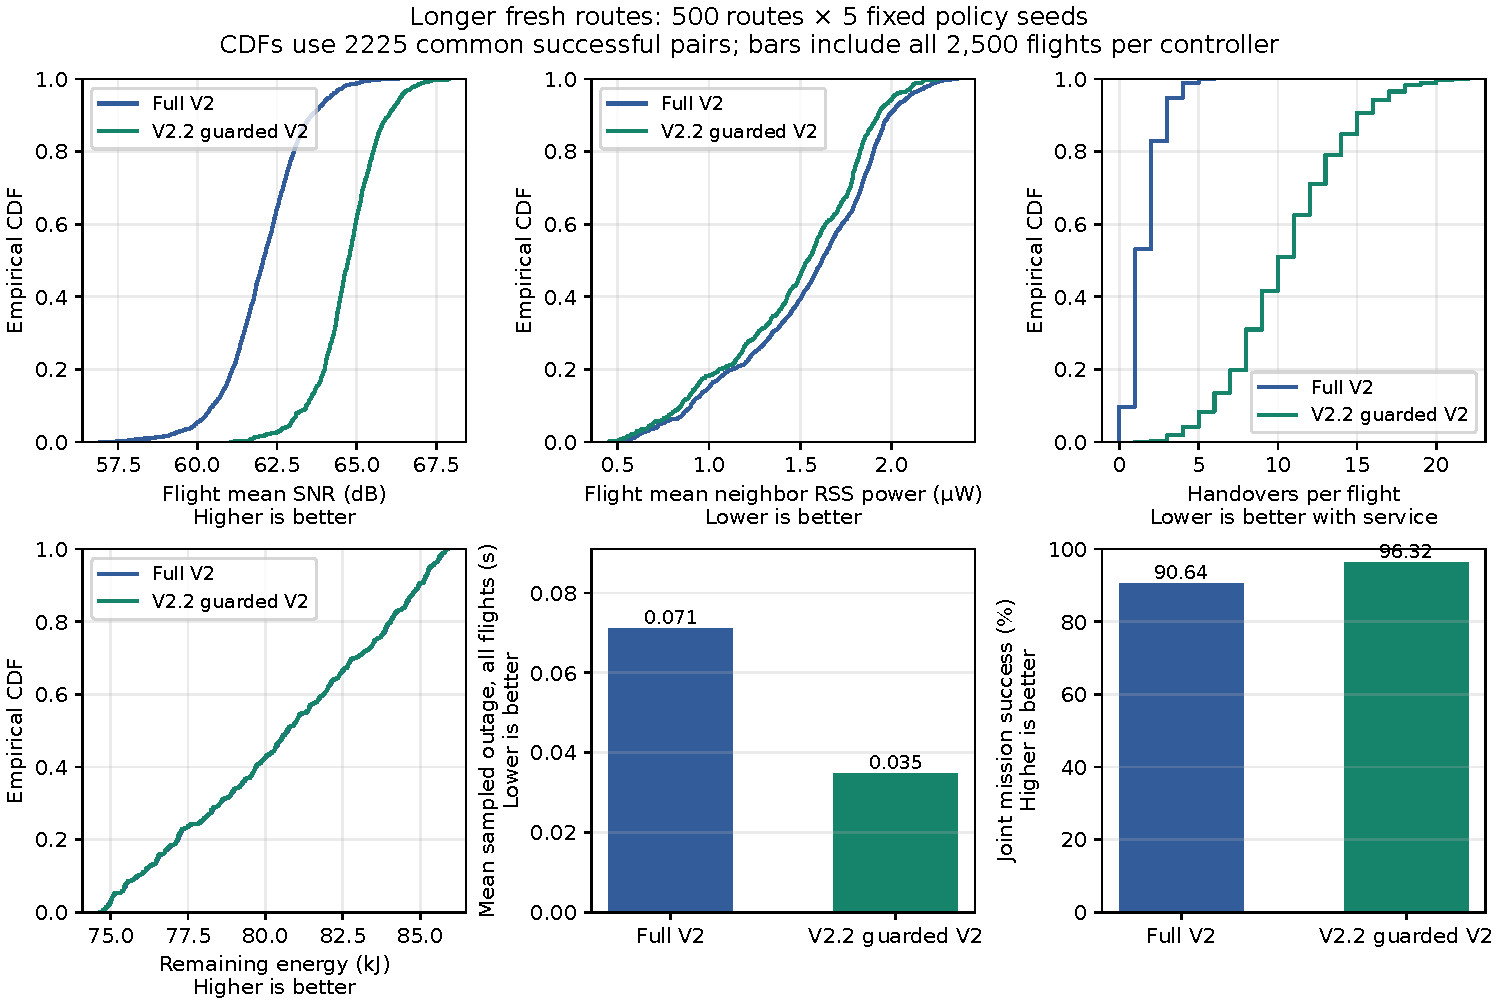
\includegraphics[width=.97\textwidth]{../results/thesis_metrics_v22/analysis/metric_comparison_longer_test.pdf}
\caption{Longer fresh route metrics. CDFs compare per flight values on common successes; bars include all flights. SNR is a per flight mean, all neighbor power is the explicit source equation proxy, and remaining energy uses V2 accounting. Sampled outage ends at the first violation and is censored. These are not reconstructed source figure distributions.}
\end{figure*}
